\chapter{Analisi lessicale: espressioni regolari, DFA, NFA}
\section{analisi lessicale}
partiamo dalla definizione
\dfn{Analisi lessicale}{
    Riconoscere nella stringa in ingresso gruppi/sequenze di simboli che corrispondono a specifiche categorie sintattiche
}

La stringa in input,poi, è trasformata in una sequenza di simboli astratti, detti \textbf{token}, si analizzi la figura:
\begin{center}
    \begin{tikzpicture}[node distance=2cm]

        % Nodes
        \node (inizio) [startstop] {Programma in input};
        \node (algorithm) [process, below of=inizio] {analizzatore lessicale};
        \node (fin) [startstop, below of=algorithm] {lista di tolen};
        
        % Arrows
        \draw [arrow] (inizio) -- (algorithm);
        \draw [arrow] (algorithm) -- (fin);
        
\end{tikzpicture}
\end{center}

\subsection{token}
\dfn{Token}{
    un token è una coppia (nome, valore), dove:
    \begin{itemize}
        \item nome: simbolo astratto che rappresenta una categoria semantica
        \item Valore: una sequenza di simboli del testo in ingresso
    \end{itemize}
}
Esempietto:
\esempio{
    Un esempio di token è $\inside{Ide, x1}$, dove:
    \begin{itemize}
        \item $Ide$: è l'informazione che identifica una classe di token
        \item $x1$: è l'infomrazione che identifica lo specifico token 
        \item 
    \end{itemize}
}
Siano inoltre tali definizioni
\dfn{Pattern}{
    è la descrizione generale della forma dei valori di una classe di token
}
\esempio{
    Sia $(x\mid y)(x\mid y\mid 0\mid 1)^*$ un'espressione regolare per rappresentare un Pattern, un esempio di stringa è
}

\dfn{
    lessema
}{
    si definisce \textbf{lessema} una stringa istanza di un pattern
}
\esempio{
    nel nostro esempio $x1$ è un'istanza di un pattern
}

vedremo che ad ogni nome di categoria sintattica è associato un pattern che specifica i possibili valori che possono essere presi per quel nome, come lessemi

\esempio{
    dalla strinfa $C$ si ha:
    \begin{center}
        \texttt{if}$(x==0)$ \texttt{printf("zero")}
    \end{center}

    un analizzatore lessicale potrebbe produrre la seguente sequenza di token:
    \begin{itemize}
        \item $\inside{\text{\texttt{if}}}$
        \item $\inside{\text{\texttt{(}}}$
        \item $\inside{ide, x}$
        \item $\inside{Operel, ==}$
        \item $\inside{const-num, 0}$
        \item $\inside{\text{\texttt{)}}}$
        \item $\inside{Ide, \text{\texttt{printf}}}$
        \item $\inseide{\text{\texttt{(}}}$
        \item $\inside{const-string, \text{\texttt{zero}}}$
        \item $\inside{\text{\texttt{)}}}$
    \end{itemize}
}
In realtà, normalmente lo scanner \red{associa agli identificatori un indirizzo della tabella dei simboli}, quindi  $\inside{ide, x}$ è in realta  $\inside{ide, \text{puntatore alla tabello dei simboli}}$

\subsection{espressioni regolari}
\dfn{espressioni regolari}{
    fissato un alfabeto $A =\{a_1,a_2,\dots,a_n\}$, definiamo le espressioni regolari su $A$ con la seguente $BNF$
    \[
        r::= \varnothing\mid\epsilon\mid a\mid r\cdot r\mid r|r\mid r^*    
    \]
}
\nt{
    Si tenga presente che questa è una sintassi astratta ambigua, ci vorrebbero le parentesi per disanbiguare, tuttavia noi assumiamo che:
    \begin{itemize}
        \item la concatenazione, disgiunzione e ripetizione associano a \texttt{sx}
        \item la precedenza tra gli operatori sia: \texttt{* > $\cdot$ > |}
        \item la concatenazione $\cdot$ è di solito omessa
    \end{itemize}

    Per cui, ad esempio, $b*a|c$ corrisponde all'albero sintattico:
    \begin{center}
        \begin{tikzpicture}
            \Tree[
                .$|$
                [
                    .$\cdot$
                    [
                        .$*$
                        b
                    ]
                    a
                ]
                c
            ]
        \end{tikzpicture}
    \end{center}
    
    Quindi secondo una sintassi non ambigua: $(((b)^*)\cdot(a))|(c)$ 
}
\subsubsection{linguaggio denotato da una espressione regolare}
\dfn{}{
    dato l'alfabeto $A$, definiamo la funzione:
    \[
        \mathcal{L}:\text{\texttt{Exp-Reg}}\to\mathcal{P}(A^*)
    \]
    Come segue:
    \\
    \begin{math}
        \begin{array}{l}
            \mathcal{L}[\varnothing]=\varnothing\text{ linguaggio vuoto}\\
            \mathcal{L}[\epsilon]=\{\epsilon\} \text{ linguaggio che contiene solo la stringa vuota}\\
            \mathcal{L}[a]=\{a\}\\
            \mathcal{L}[r_1\cdot r_2] = \mathcal{L}[r_1] \cdot \mathcal{L}[r_2]\\
            \mathcal{L}[r_1|r_2] = \mathcal{L}[r_1]\cup \mathcal{L}[r_2]\\
            \mathcal{L}[r^*]=(\mathcal{L}[r])^*
            
        \end{array}    
    \end{math}
}

\nt{
    Si ricordi che:

    \begin{math}
        \begin{array}{l}
                L_1\cdot L_2 =\{xy\mid x\in L_1,y\in L_2\}\\
                L_1\cup L_2 =\{x\mid x\in L_1\text{\texttt{ or }}x\in L_2\}\\
                L^\circ =\{\epsilon\}\\
                L^{n+1} = L\cdot L^n\\
                L^*=\bigcup_{n\geq0}L^n

        \end{array}
    \end{math}
}
\subsubsection{linguaggio regolare}
\dfn{Linguaggio regolare}{
    un linguaggio $L\subseteq A^*$ è definito regolare sse $\exists$ una espressione regolare $r$ tale che:
    \[
        L=\mathcal{L}[r]    
    \]
    
}
\mprop{}{
     ogni linguaggio finito è regolare   
    }
\esempio{
    Sia $L=\{a,bc\}$ con $r=a\mid bc$
    si ha che:
    \[
        
            \mathcal{L}[a\mid bc] = \mathcal{L}[a]\cup \mathcal{L}[bc] =\{a\}\cup \mathcal{L}[b]\cdot \mathcal{L}[c] = \{a\}\cup\{b\}\cdot\{c\} = \{a,bc\}=L
    \]
}

Si osservi che esistono anche linguaggi regolari infiniti:
\[
\begin{aligned}
    \mathcal{L}[a^*b] &= \mathcal{L}[a^*] \cdot \mathcal{L}[b] = (\mathcal{L}[a])^* \cdot \mathcal{L}[b] \\
    &= \{a\}^* \cdot \{b\} = \bigcup_{m \geq 0} \{a^m\} \cdot \{b\} \\
    &= \{\epsilon, a, aa, \ldots\} \cdot \{b\} = \{a^m b \mid n \geq 0\}.
\end{aligned}
\]

\[
\begin{aligned}
    \mathcal{L}[a \mid a^*b] &= \mathcal{L}[a] \cup \mathcal{L}[a^*b] = \{a\} \cup \{a^m b \mid n \geq 0\}.
\end{aligned}
\]

\[
\begin{aligned}
    \mathcal{L}[(a \mid b) \cdot b^*] &= \mathcal{L}[a \mid b] \cdot \mathcal{L}[b^*] = (\mathcal{L}[a] \cup \mathcal{L}[b]) \cdot (\mathcal{L}[b])^* \\
    &= \{a, b\} \cdot \{b\}^* = \{a b^m \mid n \geq 0\} \cup \{b^n \mid n \geq 1\}.
\end{aligned}
\]

\ex{espressioni regolari}{
    $A=\{0,1\}$
    \begin{itemize}
        \item $0^*10^*$
        
        Con $\quad L_2\{w\in A^*\mid A^*\mid w \text{ contiene un solo }1\}$
        \item $(0\mid 1)^*001(0\mid1)^*$
        
        Con $\quad L_1\{w\in A^*\mid A^*\mid w \text{ contiene un solo }1\}$
        \item $1^*(011^*)^*$
        
        Con $\quad L_3 =\{w\in A^*\mid w \text{ contiene }001 \text{ come sottostringa}\}$
    \end{itemize}
}
\subsubsection{altri operatori ausiliari}
% TODO non ho voglia 
\dfn{}{}

\subsection{equivalenza tra espressioni regolari}
\dfn{
    equivalenza
}{
    Due espressioni regolari $r$ ed $s$ sono \textbf{equivalenti} sse $\mathcal{L}[r]=\mathcal{L}[s]$ (cioè demotano lo stesso linguaggio) e lo denotiamo con $r\equiv s$
}

Esistono molte leggi per $\equiv$, alcune sono le seguenti 
\[
r | s \simeq s | r \quad \text{(1 è commutativa)}
\]
\[
r | (s | t) \simeq (r | s) | t \quad \text{(1 è associativa)}
\]
\[
z | z \simeq z \quad \text{(1 è idempotente)}
\]
\[
z \cdot (s \cdot t) \simeq (z \cdot s) \cdot t \quad \text{($\cdot$ è associativa)}
\]
\[
\varepsilon \cdot z \simeq z \cdot \varepsilon \simeq z \quad \text{($\varepsilon$ è l'elemento neutro per $\cdot$)}
\]
\[
(r^*)^* \simeq r^* \quad \text{(* è idempotente)}
\]
\[
r (s | t) \simeq r s | r t \quad \text{(distribuisce a sinistra su |)}
\]
\[
(r | s) t \simeq r t | s t \quad \text{(distribuisce a destra su |)}
\]

In alcuni casi è facile dimostrare queste leggi:
\[
    \mathcal{L}[r|s] =\mathcal{L}[r]\cup\mathcal{L}[s]=\mathcal{L}[s]\cup\mathcal{L}[r] = \mathcal{L}[s|r]    
\]
\[
    \mathcal{L}[r|r]=\mathcal{L}[r]\cup \mathcal{L}[r]=\mathcal{L}[r]
\]
\[
    \mathcal{L}[r\epsilon] = \mathcal{L}[r]\cdot\{\epsilon\}=\mathcal{L}[r]
\]
\[
    \mathcal{L}[\varnothing^*] = (\mathcal{L}[\varnothing]) = \varnothing^*=\varnothing^0\cup\varnothing^1\cup\varnothing^2\dots=\{\epsilon\}\cup\varnothing\cup \varnothing=\{\epsilon\}=\mathcal{L}[\epsilon]    
\]
\[
    \mathcal{L}[r\dot \varnothing]=\mathcal{L}[r]\cdot\mathcal{L}[\varnothing]=\mathcal{L}[r]\cdot\varnothing=\varnothing=\mathcal{L}[\varnothing]    
\]

Le espressioni regolari servono per specificare il pattern di una categoria sintattica, ovvero la forma dei possibili lessemi, tuttavia occorre riconoscere se una certa sequenza in ingresso è un lessema per una certa categoria sintattica. A questo ci vengono in aiuto gli automi a stati finiti

\section{Automi a stati finiti}
Un \textbf{automa a stati finiti} (o DFA, deterministic finite automaton, per la versione deterministica) è un modello computazionale utilizzato per rappresentare e analizzare linguaggi regolari. È un \red{dispositivo astratto che processa stringhe di simboli e decide se appartengono o meno a un linguaggio}

Si può immaginare il DFA come una automa ideale dotato di una testina di lettura, una sequenza di simboli in input da leggere e un sistema di stati, del tipo

%todo aggiungere immagine 

Dove inizialmente 
\begin{itemize}
    \item la testina di lettura è posizionata sul primo carattere dell'input
    \item e vi è un controllo su sullo stato iniziale $q_0$
\end{itemize}

E funziona ciclicamente nel modo seguente:
\begin{itemize}
    \item leggi il carrattere in input e in baso allo stato in cui si trova decide:
    \begin{itemize}
        \item di cambiare di stato
        \item di spostare la testina sull'input successivo
    \end{itemize}
    FINO A CHE:
    \item ha finito di leggere l'input (e riconosce la stringa)
    \item non ha riconosciuto la stringa 
\end{itemize}

\subsection{diagrammi di transazione}
il funzionamento di un automa finito  è ben descritto dai cosiddetti \textbf{diagrammi di transizione}

\begin{center}
    \begin{tikzpicture}[shorten >=1pt, node distance=2cm, on grid, auto] 
    \node[state, initial] (q_0)   {$q_0$}; 
    \node[state, accepting] (q_1) [right=of q_0] {$q_1$}; 
     
    \path[->] 
     (q_0) edge [bend left] node {a} (q_1)
     (q_1) edge [bend left] node {a} (q_0);
 \end{tikzpicture}
\end{center}

Riconoscere una stringa $w$ significa trovare un cammino etichettato $w$ sul grafo a partire dallo stato iniziale che finisce su uno stato finale 
\[
    L =\{a^{2n+1}\mid n\geq 0\} = \{a^n\mid n \text{ è dispari}\} = \mathcal{L}[a(aa)^*]    
\]
\esempio{
    \begin{itemize}
        \item Primo esempio:
        Sia $L=\{w\in \{0,1\}^*\mid \text{ in  }w\text{ il numero di }0\text{ e }1\text{ è sempre pari}\}$

        Il suo automa è:
        \begin{center}
            \begin{tikzpicture}
            \node[state, initial, accepting] (q0) {$q_0$};
            \node[state, right of=q0] (q1) {$q_1$};
            \node[state, below of=q0] (q2) {$q_2$};
            \node[state, right of=q2] (q3) {$q_3$};
            
            \path[->]
            (q0) edge [bend left] node {$1$} (q1)
            (q1) edge [bend left] node {$1$} (q0)

            (q2) edge [bend left] node {$1$} (q3)
            (q3) edge [bend left] node {$1$} (q2)

            (q2) edge [bend left] node {$0$} (q0)
            (q0) edge [bend left] node {$0$} (q2)

            (q1) edge [bend left] node {$0$} (q3)
            (q3) edge [bend left] node {$0$} (q1)
            
        \end{tikzpicture}
        \end{center}
        \item secondo esempio
        
        Sia $L=\mathcal{L}[(a|b)^*ba]$

        il suo automa è:
        \begin{center}
            \begin{tikzpicture}
                \node[state, initial] (q0) {$q_0$};
                \node[state, right of=q0] (q1) {$q_1$};
                \node[state, accepting, right of=q1] (q2) {$q_2$};

                \path[->]
                    (q0) edge[loop below] node {$a$} (q0)
                    (q0) edge[loop ] node {$a$} (q0)
                    (q0) edge[below] node {$b$} (q1)
                    (q1) edge[below] node {$a$} (q2);
            \end{tikzpicture}
        \end{center}

        Si noti che $ba\in L[M]$ (ovvero $ba$ appartiene al linguaggio riconosciuto dall'automa $M$)  perché esiste un cammino da $q_0$ a $q_2$ etichettato $ba$

        Questo linguaggio è \red{non deterministico}:
        \begin{itemize}
            \item $(q_0, b)$ offre 2 mosse o su $q_0$ o su $q_1$
            \item $(q_1, b)$ non offre mosse
            \item $(q_2, a/b)$ non offre mosse 
        \end{itemize}

        \item terzo esempio:
        
        Sia $L[M]=\mathcal{L}[a^*b^*]$

        Riconosciuto dal seguente automa:
        \begin{center}
            \begin{tikzpicture}
                \node[state, initial] (q0) {$q_0$};
                \node[state, accepting, right of=q0] (q1) {$q_1$};

                \path[->]
                    (q0) edge[loop below] node {$a$} (q0)
                    (q0) edge[above] node {$\epsilon$} (q1)
                    (q1) edge[loop above] node {$b$} (q1);
            \end{tikzpicture}
        \end{center}

        Che \red{nondeterministico} perché è possibile spostarsi dallo stato $q_0$ allo stato $q_1$ senza leggere l'input. 
        
        Se vogliamo un automa deterministico:
        \begin{center}
            \begin{tikzpicture}
                \node[state, accepting, initial] (q0) {$q_0$};
                \node[state, accepting, right of=q0] (q1) {$q_1$};
                \node[state, right of=q1] (q2) {$q_2$};

                \path[->]
                    (q0) edge[loop below] node {$a$} (q0)
                    (q0) edge[above] node {$b$} (q1)
                    (q1) edge[loop above] node {$b$} (q1)
                    (q1) edge[above] node {$a$} (q2)
                    (q2) edge[loop above] node {$b/a$} (q2);
            \end{tikzpicture}
        \end{center}   
        Dove $q_2$ è uno stato pozzo d'errore. Inoltre da ogni stato per ognuno dei due simboli ($a$ e $b$), esce una e una sola transizione e non vi sono transizioni $\epsilon$

        
    \end{itemize}
}
\subsection{Automi a stati finiti non deterministico}
Adesso formalizziamo la definizione
\dfn{Automi a stati finiti non deterministici}{
    Si defisnisce  \textbf{NFA o automa a stati finiti non deterministico} una quintupla $(\Sigma, Q, \delta, q_0, F)$ dove:
    \begin{itemize}
        \item $\Sigma$ è un alfabeto finito di simboli in input
        \item $Q$ è un insieme finito di stati
        \item $q_0\in Q$ è lo stato iniziale 
        \item $F\subseteq Q$ è l'insieme degli stati finali
        \item $\delta$ è la funzione di transizione con tipo
        
        \[
            \delta : Q\times (\Sigma\cup\{\epsilon\})\to \mathcal{P}(q)    
        \]
    \end{itemize}
    
}
Esempietto:
\esempio{
    \[
        \Sigma = \{a, b\} \quad Q = \{q_0, q_1, q_2\} \quad q_0 \text{ iniziale} \quad F = \{q_2\}
    \]

    \[
        \delta =
        \begin{array}{c|c|c|c}
            & a & b & \varepsilon \\
            \hline
            q_0 & \{q_0\} & \{q_0, q_1\} & \varnothing \\
            q_1 & \{q_2\} & \varnothing & \varnothing \\
            q_2 & \varnothing & \varnothing & \varnothing \\
        \end{array}
    \]

    \vspace{1cm}

    Si può vedere la seguente tabella mutarsi in automa
    \vspace{0.5cm}

    \begin{center}
        \begin{tikzpicture}[shorten >=1pt, node distance=2.5cm, on grid, auto]
        % Stati
        \node[state, initial] (q0) {$q_0$};
        \node[state] (q1) [right=of q0] {$q_1$};
        \node[state, accepting] (q2) [right=of q1] {$q_2$};

        % Transizioni
        \path[->]
        (q0) edge[loop above] node {$a$} ()
            edge[loop below] node {$b$} ()
            edge[above] node {$b$} (q1)
        (q1) edge node {$a$} (q2);
        \end{tikzpicture}
    \end{center}

}
\subsection{Linguaggio riconosciuto/accettato}
Fornisco prima, formalmente, prima alcune definzioni:

\dfn{mossa}{
    Si definisce \textbf{mossa} da uno stato $q$ ad uno stato $q'$ leggendo un simbolo $\sigma$ dall'input e la si denota con $\vdash_n$ tale derivazione (attraverso regole di inferenza logica):
    \[
        \frac{q'\in\delta(q, \sigma)}{(q,\sigma w)\vdash_n (q',w)} \text{ con }\begin{array}{l}
            \sigma\in \Sigma\cup\{\epsilon\}\\
            w\in\Sigma^*
        \end{array}   
    \]
}

Da cui discende la definizione di cammino
\dfn{cammino (chiusura riflessiva e transitiva di $\vdash_n$)}{
    Si definisce cammino da uno stato $q$ ad uno stato $q''$ tale derivazione:
    \[
        \frac{(q,w)\vdash_n^*(q',w')\quad (q',w')\vdash_n (q'',w'')}{(q,w)\vdash_n^*(q'',w'')}    
    \]

    Inoltre si ha:
    \[
        \frac{}{(q,w)\vdash_N^*(q,w)}    
    \]
}

da cui discenda la definizione di riconoscimento
\dfn{riconoscimento}{
    Una stringa $w$ si definisce \textbf{riconosciuta} se è vera tale proposizione:
    \[
        w\in L[N]\iff \exists q\in F.(q_0,w)\vdash_n^* (q,\epsilon)    
    \]
}

e da cui discende la definizione di linguaggio accettato
\dfn{linguaggio accettato}{
    Un lingaggio $L$ si definisce \textbf{accettto da un automa $N$}, indicato con $L[N]$, è
    \[
        L[N] =\{w\in\Sigma^*\mid \exists q\in F. (q_0, w)\vdash_n^* (q,\epsilon)\}       
    \]
}

\nt{
    due NFA $N_1$ e $N_2$ si dicono \textbf{equivalenti} sse accettano lo stesso linguaggio, cioè se $L[N_1]= L[N_2]$
}

Gli NFA sono comodi, ovvero facili da costruire, tuttavia sono \red{inefficienti}, infatti accettare $w$ significa cercare un cammino su un grafo nondeterministico, il che porta a tante potenziali strade alternative.

In alternativa si possono costruire dei DFA ovvero automi deterministici a stati finiti 

\subsection{Automi a stati finiti deterministici}
Un DFA a differenza degli NFA ha le seguenti caratteristiche:
\begin{itemize}
    \item $\delta (q,\sigma)$ è sempre un singoletto (solo una mossa possibile)
    \item non ci sono mosse $\epsilon$
\end{itemize}
E questo implica
\begin{itemize}
    \item una scansione completa dell'input garantita
    \item in un tempo $O(|w|)$ sappiamo se $w$ è accettata o meno
    \item difficile da definire
\end{itemize}

Introduciamo la definizione formalmente
\dfn{
    Automi deterministici a stati finiti 
}{
    Un \textbf{automa deterministico a stati finiti} (DFA) è una quintupla $(\Sigma, Q, \delta, q_0, F)$ dove:
    \begin{itemize}
        \item $\Sigma$ è un alfabeto finito di simboli in input
        \item $Q$ è un insieme finito di stati
        \item $q_0\in Q$ è lo stato iniziale 
        \item $F\subseteq Q$ è l'insieme degli stati finali
        \item $\delta$ è la funzione di transazione con tipo
        
        \[
            \delta : Q\times \Sigma\to Q    
        \]
        e si ha che $(q,\sigma) = q'$
    \end{itemize}
}

Si osservi che
\clm{}{}{
    Un DFA è un particolare tipo di NFA tale che:
    \begin{itemize}
        \item $\forall q\in Q.\;\delta(q,\epsilon)=\varnothing$
        
        Ovvero \red{non ci sono transizioni $\epsilon$}
        \item $\forall \sigma\in \Sigma.\;\forall q\in Q.\;\exists q'\in Q.\;\delta(q,\sigma)=\{q'\}$
        
        Ovvero l'insieme delle mosse possibile è sempre un singoletto
    \end{itemize}

    \begin{center}
       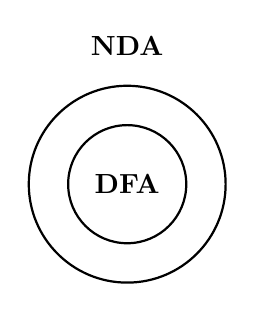
\begin{tikzpicture}
        % Cerchi per gli automi
        \draw[thick] (0, 0) circle (0.75cm) node[pos=0, yshift=0cm] {\textbf{DFA}};
        \draw[thick] (0, 0) circle (1.25cm) node[pos=0, yshift=1.75cm] {\textbf{NDA}};
    \end{tikzpicture} 
    \end{center}
    
}

Si vuole ora dimostrare che i \red{DFA sono tanto espressivi quanto gli NFA}, sebbene siano un loro sottoinsieme proprio

\mprop{}{
    Per ogni NFA, è prossibile costruire un DFA ad esso equivalente

}
\dimostrazione{
    Occorre seguire contemporaneamente tutti i possibili cammini alternativi dell'NFA di modo che gli stati del DFA che andranno a costruire sono costituiti sa insiemi di stati dell'NFA
}
Per dimostrare questa cosa occorre prima introdurre diversi concetti

\subsubsection{$\epsilon$-closure}

\dfn{$\epsilon$-closure}{
    L'\(\epsilon\)-closure di uno stato \(q \in Q\), denotata come \(\epsilon\text{-closure}(q)\), è definita come l'insieme degli stati \(q'\) tali che esiste un cammino da \(q\) a \(q'\) usando solo transizioni \(\epsilon\), inclusivamente \(q\) stesso.

    In simboli:
    \[
        \epsilon\text{-closure}(q) = \{ q' \in Q \mid q \xrightarrow{\epsilon^*} q' \},
    \]

    In altre parole si puo defnire come il minimo insieme che rispettˆa le seguenti regole:
    \[
        \frac{}{\{q\}\subseteq \epsilon\text{-closure}(q)}\quad\frac{p\in \epsilon\text{-closure}(q)}{\delta(p,\epsilon)\subseteq \epsilon\text{-closure}(q)}    
    \]

}
nel caso abbiamo un insieme $P$ di nodi allarghiamo la definizione di $\epsilon\text{-closure}$ a quella di:
\[
    \epsilon\text{-closure}(P) = \bigcup_{p\in P}\epsilon\text{-closure}(p)
\]

\esempio{
    Considera il seguente NFA:
    \begin{itemize}
        \item Stati: \(Q = \{q_0, q_1, q_2\}\)
        \item Transizioni:
        \begin{itemize}
            \item \(\delta(q_0, \epsilon) = \{q_1\}\)
            \item \(\delta(q_1, \epsilon) = \{q_2\}\)
            \item \(\delta(q_2, a) = \{q_2\}\)
        \end{itemize}
    \end{itemize}
    Il calcolo dell'\(\epsilon\)-closure è presto fatto:
    \begin{itemize}
        \item \(\epsilon\text{-closure}(q_0)\):
        \begin{itemize}
            \item Da \(q_0\), puoi raggiungere \(q_1\) attraverso una transizione \(\epsilon\)
            \item Da \(q_1\), puoi raggiungere \(q_2\) attraverso un'altra \(\epsilon\)
        \end{itemize}
        Quindi: \(\epsilon\text{-closure}(q_0) = \{q_0, q_1, q_2\}\)
        \item  \(\epsilon\text{-closure}(q_1)\):
        \begin{itemize}
            \item  Da \(q_1\), puoi raggiungere \(q_2\) attraverso una transizione \(\epsilon\)
        \end{itemize}
        Quindi: \(\epsilon\text{-closure}(q_1) = \{q_1, q_2\}\)
        \item \(\epsilon\text{-closure}(q_2)\):
        \begin{itemize}
            \item \(q_2\) non ha transizioni \(\epsilon\) in uscita
        \end{itemize}
        Quindi: \(\epsilon\text{-closure}(q_2) = \{q_2\}\)
    \end{itemize}

}

Qui è presentato l'algoritmo per calcolare la $\epsilon$-closure:
\begin{algorithm}
    \caption{$\epsilon$-closure}
    \KwIn{Stato $p$}
    \KwOut{insieme di stati raggiungibili da $p$ con mosse $\epsilon$}

    $T\gets P$\tcp*{inizalizzazione}
    $\epsilon$-closure($p$) = P\tcp*{inizalizzazione}

    \While{$T\neq \varnothing$}{
        scegli un $r\in T$ e rimuovilo da $T$\;
        \ForEach{$s\in\delta(r,\epsilon)$}{
            \If{$s\neq\epsilon$-closure($p$)}{
                add $s$ to $\epsilon$-closure($p$)\;
                add $s$ to T\;
            }
        }
    }
\end{algorithm} 
\clm{}{}{
    usando le $\epsilon$-closure. si può definire il linguaggio riconosciuto da un NFA in modo elegante. 
    
    Definiamo la seguente funzione
    \[
        \hat{\delta}:Q\times \Sigma^* \mathcal{Q}(P)
    \]
    per in induzione
    \[
        \hat{\delta}(q,\epsilon) = \epsilon\text{-closure}(q)
    \]
    \[
        \hat{\delta}(q,xa) = \epsilon\text{-closure}(q) \text{ dove }P=\{p\in Q\mid \exists r\in \hat{\delta}(q,x)\land p\in (r,a)\}
    \]
    

    Pertanto si può dimostrare (dimostrazione difficile) che:
    \[
        w\in L[N] \iff \exists p \in F t.c. p\in \hat{\delta}(q_0,w)
    \]
}
\subsubsection{funzione mossa}
\dfn{
    funzione mossa
}{
    Si definisce la \textbf{funzione mossa} come estensione della funzione di transizione $\delta$ di un NFA come:
    \[
        \begin{array}{l}
            mossa:\mathcal{P}(Q)\times \Sigma\to \mathcal{P}(Q)\\
            mossa(P,a) = \bigcup_{p\in P}\delta (p,a)
        \end{array}
        
    \]
    Cioe l’insieme delle mosse $a$ da un insieme di nodi $P$ e l’unione di tuˆe le mosse $a$ di ogni nodo dell’insieme. `
}

\subsubsection{funzione transazione}
\dfn{funzione transizione}{
    Si definisce \textbf{transizione} e la si denota con $\Delta$ tale funzione:
    \[ 
        \Delta(A,b)=\epsilon\text{-closure}(mossa(A,b)) 
    \]
    Con $A$ un insieme di stati e $b$ una transizione
}

\subsubsection{costruzione per sottoinsiemi}
Qua di seguito l’algoritmo per la costruzione di sottoinsiemi, che serve per passare da un NFA a un DFA equivalente










\begin{algorithm}
    Sia $N=(\Sigma, Q,\delta,q_0,F)$ un NFA\;
    $S\gets\epsilon\text{-closure}$\tcp*{stato iniziale del DFA}
    $T=\{S\}$\tcp*{$T$ è il l'insieme degli stati del DFA}
    \While{c'è un $P\in T$ non marcato}{
        marca $P$\;
        \ForEach{$a\in\Sigma$}{
            $R\gets \epsilon\text{-closure}(mossa(P,a))$\;
            \If{$R\notin T$}{
                add $R$ to $T$\tcp*{$R$ non ha marca}
                definisci $\Delta(P,a) = R$\;
        }
    }
}
\end{algorithm}






Si può notare come l'algoritmo che definisce la funzione di transizione (vista poch'anzi) rispett‹a le limitazioni dei DFA: non ci sono mosse epsilon e per ogni cara‹ere dell’alfabeto esiste una ed
una sola mossa in qualunque stato
\esempio{
    Consideriamo l’NFA seguente (relativo all’espressione regolare $(a|b)^*ab)$:
    \begin{tikzpicture}
        \node[state, initial] (q0) {$q_0$};
        \node[state] (q1) [right=of q0] {$q_1$};
        \node[state, accepting] (q2) [right=of q1] {$q_2$};

        % Transizioni
        \path[->]
        (q0) edge[loop above] node {$a$} ()
            edge[loop below] node {$b$} ()
            edge[above] node {$b$} (q1)
        (q1) edge node {$a$} (q2);
    \end{tikzpicture}

    Vogliamo ora trovare un DFA equivalente ad esso, applichiamo l’algoritmo di costruzioni per sottˆoinsiemi:
    \begin{itemize}
        \item calcoliamo lo stato iniziale $S=\epsilon\text{-closure}(q_0)$, che è $S=q_0$. 
        \item Creiamo $T$ e gli inseriamo $S$ marcandolo
        \item Per ogni simbolo dobbiamo calcolare $\epsilon\text{-closure}(mossa(P,a))$, ma visto che l'alfabeto è $\{a,b\}$ lo facciamo 2 volte:
        \begin{itemize}
            \item per il carattere $a$ calcoliamo con $P=S=\{q_0\}$:
            \[
                \begin{array}{l}
                    R = \epsilon\text{-closure}(mossa(P,a)) = \epsilon\text{-closure}\left(\bigcup_{p\in\{q_0\}}\delta (p,a)\right)\\
                    =\epsilon\text{-closure}(\delta(q_0,a)) =\epsilon\text{-closure}(\{q_0\}) =\{q_0\}
                \end{array}
                 
            \]
            Si definisca $\delta(S,a)=\{q_0\}$ e visto che $\{q_0\}\in T$ non lo andiamo a ri-aggiungere
            \item per il carattere $a$ calcoliamo con $P=S=\{q_0\}$:
            \[
                \begin{array}{l}
                    R = \epsilon\text{-closure}(mossa(P,b)) = \epsilon\text{-closure}\left(\bigcup_{p\in\{q_0\}}\delta (p,b)\right) \\                
                    =\epsilon\text{-closure}(\delta(q_0,b)) =\epsilon\text{-closure}(\{q_0, q_1\}) =\{q_0,q_1\}

                \end{array}
            \]
            visto che $\{q_0,q_1\}\notin T$ lo andiamo ad aggiungere
        \end{itemize}
        \item si calcoli ora con $P=\{q_0, q_1\}$ andando a calcolare la stessa cosa:
        \begin{itemize}
            \item per $a$ si ha:
            \[
                \begin{array}{l}
                    R=    \epsilon\text{-closure} (mossa(P,a)) = \epsilon\text{-closure}\left(\bigcup_{p\in\{q_0, q_1\}}\delta(p,a)\right)\\                 
                    = \epsilon\text{-closure} (\{q_0\}\cup\{ q_2\}) = \{q_0,q_2\}

                \end{array}
            \]
            quindi $\Delta(\{q_0,q_1\}, a)=\{q_0,q_2\}$. Visto $\{q_0,q_2\}\notin T$ lo aggiungiamo 
            \item  per $b$ si ha $R=\{q_0,q_1\}$. Quindi $\Delta(\{q_0, q_1\}, b) = \{q_0,q_1\}$ e non lo si raggiunge
        \end{itemize}
        \item ripetiamo per $P=\{q_0, q_2\}$ (salto i calcoli)
    \end{itemize}

    alla fine di sto ambaradam si ottiene $DFA \;N'=(\Sigma, \{\{q_0\},\{q_0,q_1\}, \{q_0,q_2\}\}, \Delta, \{q_0\}, \{q_0,q_2\})$ che in forma di diagramma di transizione e:
    \begin{center}
        \begin{tikzpicture}[shorten >=1pt, node distance=3cm, on grid, auto]

            % Stati
            \node[state, initial] (q0) {$A=\{q_0\}$};
            \node[state] (q1) [right=of q0] {$B=\{q_0, q_1\}$};
            \node[state, accepting] (q2) [below=of q1] {$C=\{q_0, q_2\}$};
        
            % Transizioni
            \path[->]
                (q0) edge[loop above] node {$a$} () % loop su q0 con "a"
                     edge[bend left] node {$b$} (q1) % da q0 a q1 con "b"
                (q1) edge[loop above] node {$b$} () % loop su q1 con "b"
                     edge[bend left] node {$a$} (q2) % da q1 a q2 con "a"
                (q2) edge[bend left] node {$b$} (q1) % da q2 a q1 con "b"
                     edge[bend left] node {$a$} (q0); % da q2 a q0 con "a"
        
        \end{tikzpicture}
            \end{center}
}

esempio bello corposo:
\esempio{
    \begin{center}
        \begin{tikzpicture}[shorten >=1pt, node distance=2cm, on grid, auto]
            % Stati
            \node[state, initial] (q0) {$q_0$};
            \node[state] (q2) [right of=q0] {$q_2$};
            \node[state, accepting] (q4) [right of=q2] {$q_4$};
            \node[state] (q1) [above of=q1] {$q_1$};
            \node[state] (q3) [right of=q1] {$q_3$};
        
            % Transizioni
            \path[->]
                (q0) edge[bend left] node {$\epsilon$} (q1)
                     edge node[below] {$b$} (q2)
                (q1) edge node {$a$} (q0)
                     edge node {$\epsilon$} (q2)
                     edge node {$\epsilon$} (q3)
                     edge node {$a$} (q4)
                (q2) edge node[below] {$b$} (q4)
                (q3) edge[bend left] node {$a$} (q4)
                (q4) edge[bend left] node {$\epsilon$} (q3);
        \end{tikzpicture}
        \end{center}
        
        si noti i seguenti calcoli
        \[
        A = \varepsilon\text{-closure}(q_0) = \{q_0, q_1, q_2, q_3\}
        \]
        \[
        \Delta(A, a) = \varepsilon\text{-closure}(\text{move}(A, a)) = \varepsilon\text{-closure}(\{q_0, q_4\}) = \{q_0, q_1, q_2, q_3, q_4\} = B
        \]
        \[
        \Delta(A, b) = \varepsilon\text{-closure}(\text{move}(A, b)) = \varepsilon\text{-closure}(\{q_2, q_3, q_4\}) = \{q_2, q_3, q_4\} = C
        \]
        \[
        \Delta(B, a) = \varepsilon\text{-closure}(\text{move}(B, a)) = \varepsilon\text{-closure}(\{q_0, q_4\}) = B
        \]
        \[
        \Delta(B, b) = \varepsilon\text{-closure}(\text{move}(B, b)) = \varepsilon\text{-closure}(\{q_2, q_4\}) = C
        \]
        \[
        \Delta(C, a) = \varepsilon\text{-closure}(\text{move}(C, a)) = \varepsilon\text{-closure}(\{ q_4\})=\{q_3, q_4\} = D
        \]
        \[
        \Delta(C, b) = \varepsilon\text{-closure}(\text{move}(C, b)) = \varepsilon\text{-closure}(\{q_4\}) = D
        \]
        \[
        \Delta(D, a) = \varepsilon\text{-closure}(\text{move}(D, a)) = \varepsilon\text{-closure}(\{q_4\}) = \varnothing = D
        \]
        \[
        \Delta(D, b) = \varepsilon\text{-closure}(\text{move}(D, b)) = \varepsilon\text{-closure}(\varnothing) = \varnothing = E
        \]
        \[
        \Delta(E, a) = \varepsilon\text{-closure}(\text{move}(E, a)) = \varepsilon\text{-closure}(\varnothing) = \varnothing = E
        \]
        \[
        \Delta(E, b) = \varepsilon\text{-closure}(\text{move}(E, b)) = \varepsilon\text{-closure}(\varnothing) = \varnothing = E
        \]
        
        \subsection*{DFA $M_N$}
        
        TODO SISTEMARE
        \begin{center}
        \begin{tikzpicture}[shorten >=1pt, node distance=3cm, on grid, auto]
            % Stati
            \node[state, initial] (A) {$A$};
            \node[state] (B) [above right=of A] {$B$};
            \node[state] (C) [below right=of A] {$C$};
            \node[state] (D) [right=of C] {$D$};
            \node[state, accepting] (E) [right=of D] {$E$};
        
            % Transizioni
            \path[->]
                (A) edge[bend left] node {$a$} (B)
                    edge[bend right] node[below] {$b$} (C)
                (B) edge[loop above] node {$a$} ()
                    edge[bend left] node {$b$} (C)
                (C) edge[bend left] node {$a$} (D)
                    edge[loop below] node {$b$} ()
                (D) edge[bend left] node {$a, b$} (E)
                (E) edge[loop below] node {$a, b$} ();
        \end{tikzpicture}
        \end{center}
}



Definiamo quindi il DFA equivalente:
\dfn{DFA quivalente}{
    Si definisce il DFA equivalente tale automa:
    \[
        M_n = (\Sigma, T,\Delta, \epsilon\text{-closure}(q_0), \mathcal{F})    
    \]
    dove $R\in \mathcal{F}\iff \exists q\in R$ con $q\in F$
}

Adesso si può dimostrare il teorema dell'equivalenza
\subsubsection{teorema d'equivalenza}

\thm{
    Bonzo-GioLaPalma
}{
    Sia $N=(\Sigma), Q,\delta,q_0, F$ un NFA  e sia $;_n$ l'automa ottenuto con la costruzione per sottoinsiemi. allora $M_n$ è un DFA e si ha che 
    \[
        L[N]=L[M_n]    
    \]
}
\dimostrazione{
    Sia \( N = (Z, \Sigma, \delta, q_0, F) \) un NFA e sia \( M_N = (\Gamma, \Sigma, \Delta, A, F') \) l'automa ottenuto con l'algoritmo.

\begin{itemize}
    \item \( M_N \) è \textbf{deterministico}: Infatti $\Delta(A, a)$ con $A\in T\land a\in \Sigma$ è definita in modo univoco 
        

    \item  Quindi mi riduco a disimostrare che $L[N]=L[M_n]$
    \begin{itemize}
        \item si osservi che per un DFA, $\epsilon$-closure$(R)=R$
        \item chiamiamo $i_m=\epsilon$-closure$(q_0)$ lo stato iniziale di $M_n$
    \end{itemize}
\end{itemize}



Vogliamo dimostrare che $\forall w\in \Sigma^*$

\[
\delta(q_0, w) = \Delta(A, w) 
\]
per induzione sulla lunghezza di $w$
\begin{itemize}
    \item \textbf{Caso base}: \( |w| = 0 \text{ cioè } (w = \epsilon) \):
    \[
    \Delta(A, \varepsilon) = \epsilon\text{-closure}(q_0) = A.
    \]
    \[
        \hat{\Delta} (i_m,\epsilon) =     \epsilon\text{-closure}(i_m)= \epsilon\text{-closure}(q_0)
    \]
    \item \textbf{Caso induttivo}:\( w = xa \) con \( x \in \Sigma^*, a \in \Sigma \)

    Per ipotesi induttiva, ammettiamo che:
    %TODO da fare cazzo
\end{itemize}


}